\documentclass[zad,zawodnik,utf8]{sinol}

\title{Krab-graf}
\id{krg}
\author{Karol Waszczuk} % Autor zadania
\pagestyle{fancy}
\iomode{stdin}
\konkurs{XIV obóz informatyczny}
\etap{początkująca}
\day{3}
\date{18.01.2017}
\RAM{32}

\usepackage{graphicx}

\begin{document}
\begin{tasktext}%

$Krab$-$grafem$ nazywamy drzewo, które posiada dwa takie wierzchołki $a$ oraz $b$, że wszystkie poniższe warunki są spełnione:

\begin{itemize}
\item wierzchołki $a$ i $b$ są połączone bezpośrednią krawędzią
\item każda ścieżka zaczynająca się w $a$ i nieprzechodząca przez $b$ ma taką samą długość oraz żadne dwie z nich nie mają wspólnej krawędzi
\item każda ścieżka zaczynająca się w $b$ i nieprzechodząca przez $a$ ma taką samą długość oraz żadne dwie z nich nie mają wspólnej krawędzi
\end{itemize}

Przy czym, mówiąc o ścieżce mamy na myśli maksymalne ścieżki, czyli takie, których długości nie możemy już wydłużyć przechodząc do sąsiedniego wierzchołka.

\begin{center}
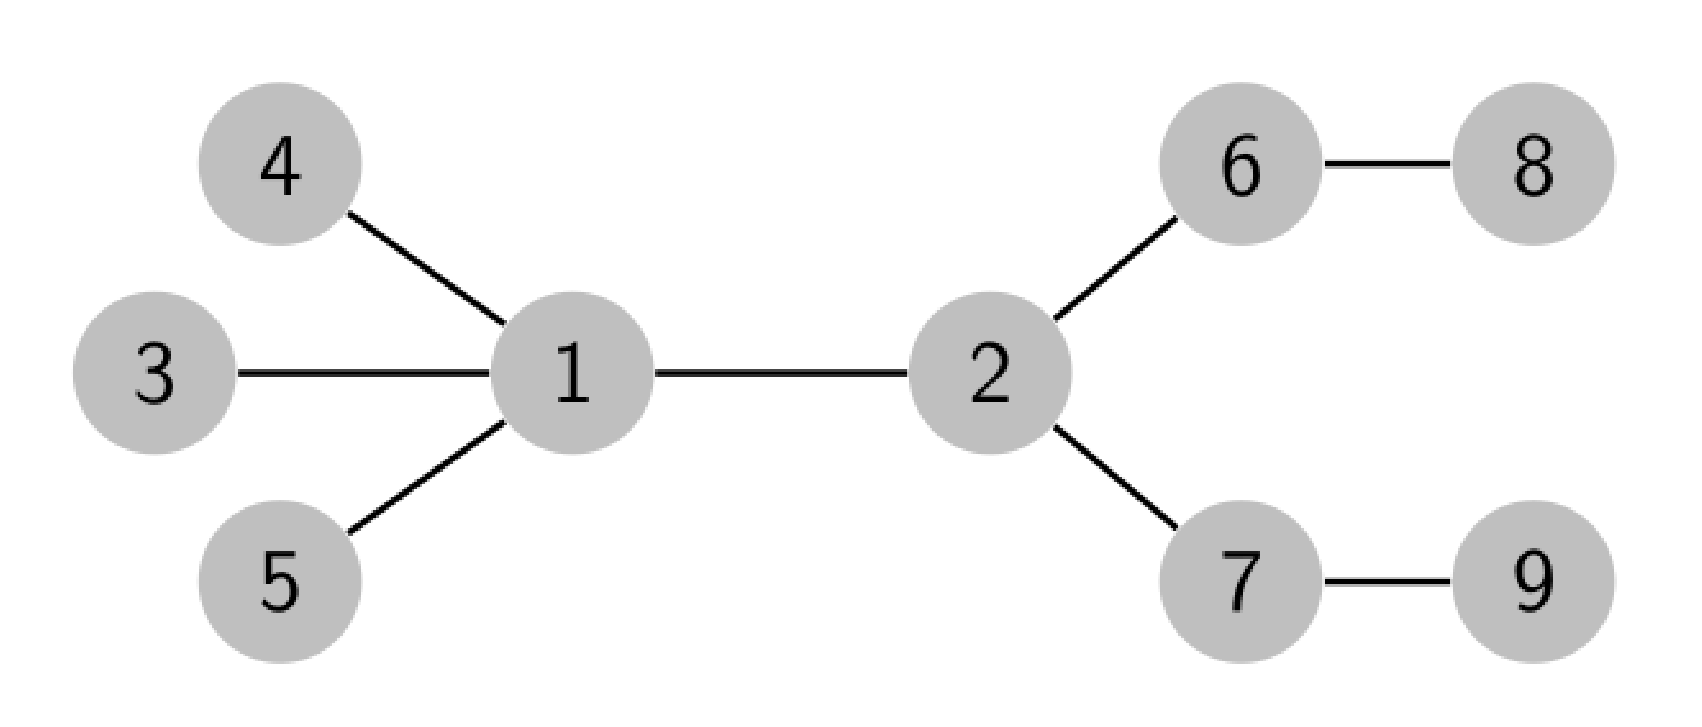
\includegraphics[height=4cm]{krab.eps}\\
\small{Tak może wyglądać przykładowy $krab$-$graf$ o $8$ wierzchołkach.}
\end{center}

Dla danego $n$-wierzchołkowego drzewa, ustal czy jest ono $krab$-$grafem$.

  \section{Wejście}

W pierwszym wierszu znajduje się jedna liczba $n$ ($2 \leq n \leq 500\ 000$) oznaczająca liczbę wierzchołków w rozpatrywanym grafie.

W każdym z kolejnych $n - 1$ wierszy znajdują się dwie liczby całkowita $a_i$ oraz $b_i$ ($1 \leq a_i, b_i \leq n, a_i \neq b_i$), oznaczające istnienie w grafie krawędzi łączącej wierzchołki $a_i$ i $b_i$. 

  \section{Wyjście}
Na standardowe wyjście należy wypisać jedno słowo \texttt{TAK}, jeśli graf z wejścia jest $krab$-$grafem$ albo \texttt{NIE} w przeciwnym przypadku.


  \section{Przykład}

   \twocol{%

       \noindent Dla danych wejściowych:

       \includefile{../in/\ID0a.in}

     }{%

       \noindent poprawnym wynikiem jest:

       \includefile{../out/\ID0a.out}

     }
 
   \twocol{%

       \noindent natomiast dla danych wejściowych:

       \includefile{../in/\ID0b.in}

     }{%

       \noindent poprawnym wynikiem jest:

       \includefile{../out/\ID0b.out}

     } 
   \twocol{%

       \noindent a dla danych wejściowych:

       \includefile{../in/\ID0c.in}

     }{%

       \noindent poprawnym wynikiem jest:

       \includefile{../out/\ID0c.out}

     }

\end{tasktext} 
\end{document}
